\documentclass[11pt, oneside]{article} 
\usepackage{geometry}
\geometry{letterpaper} 
\usepackage{graphicx}
	
\usepackage{amssymb}
\usepackage{amsmath}
\usepackage{parskip}
\usepackage{color}
\usepackage{hyperref}

\graphicspath{{/Users/telliott_admin/Dropbox/Tex/png/}}
% \begin{center} 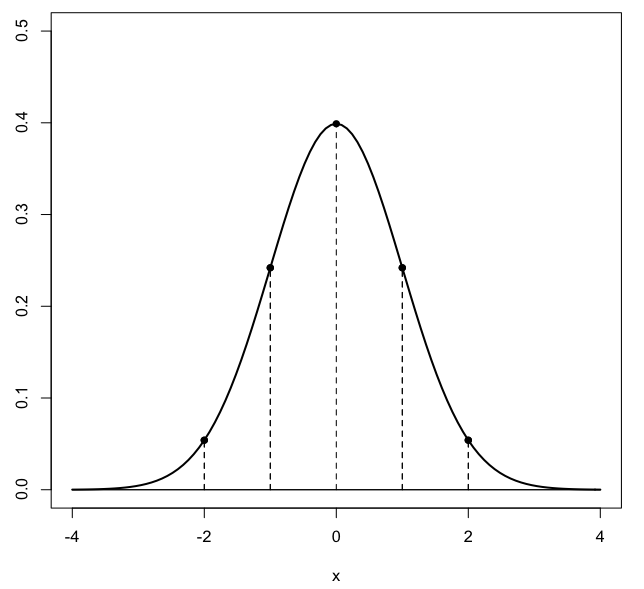
\includegraphics [scale=0.4] {gauss3.png} \end{center}

\title{Pythagorean Theorem}
\date{}

\begin{document}
\maketitle
\Large

The main result we are headed for is the Pythagorean Theorem.  Before we get there, however, it is worthwhile to continue our development of basic geometry with a discussion about right angles and right triangles.  

A right triangle is a triangle containing one right angle.  Right angles (and right triangles) are special.  We saw previously that the definition of a right angle is that two of them add up to one straight line or $180$ degrees.  Since we proved that the sum of the three angles in any triangle is equal to one straight line, by extension, the sum of angles in any triangle is also equal to two right angles.

In the figure below, the angle at vertex $P$ is a right angle.  It is common to mark a right angle with a little square, as shown, but these are a pain to draw, so I will not usually do that.  The side opposite $P$, namely $c$, is the hypotenuse.

\begin{center} 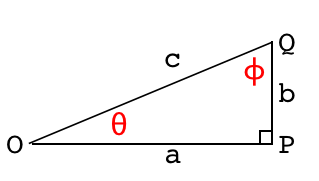
\includegraphics [scale=0.5] {angle_bisector_r3.png} \end{center}

Since the sum of angles in a triangle is equal to two right angles, the sum of the angles $\theta$ and $\phi$ above is also equal to a right angle, or 90 degrees.  Angles $\theta$ and $\phi$ are said to be complementary.  This fact is often exploited in proofs.  Here is an example we will see later on:

\begin{center} 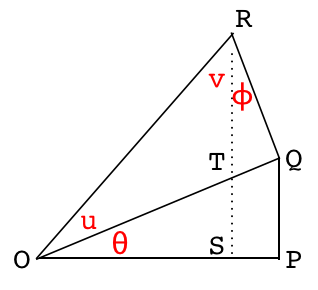
\includegraphics [scale=0.5] {angle_bisector_r4.png} \end{center}

Suppose we are given that $\angle OPQ$ and $\angle OQR$ are right angles.  We draw the altitude $RS$ and observe that the angle at vertex $S$ is a right angle.  Therefore, in triangle $ORS$, the sum $\theta + u + v$ is equal to one right angle.  At the same time, in triangle $OQR$, the sum $u + v + \phi$ is also equal to one right angle.  Therefore, $\theta = \phi$.  Further, $\triangle QRT$ and $\triangle OPQ$ are similar triangles.

\subsection*{angle bisector}

\label{sec:angle_bisector}
With that background, we now consider a classic problem:  involving angle bisectors.  Actually, before we do that, let's just show a method for constructing an angle bisector
\begin{center} 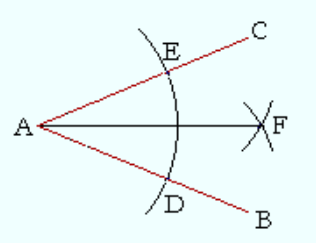
\includegraphics [scale=0.5] {angle_bisector7.png} \end{center}
To bisect angle $\angle BAC$ use the compass to mark off equal segments $AD$ and $AE$ and then mark off equal segments $DF$ and $EF$.  The line segment $AF$ bisects the angle.

Proof:  $\triangle ADF$ is congruent to $\triangle AEF$ by SSS.  Therefore, $\angle CAF = \angle BAF$.

Now, back to our problem, and the diagram below.
\begin{center} 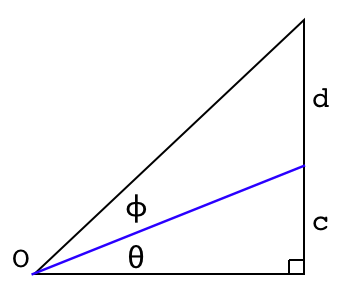
\includegraphics [scale=0.5] {angle_bisector_r0.png} \end{center}
Suppose we are given that the large triangle, and the bottom of the two smaller triangles are both right triangles.  

We draw a line joining the vertex $O$ on the left with the side opposite. This line could in general be drawn anywhere, however two interesting cases are when the angle at $O$ is bisected, or when the side opposite is bisected.

These cases are different.

\begin{center} 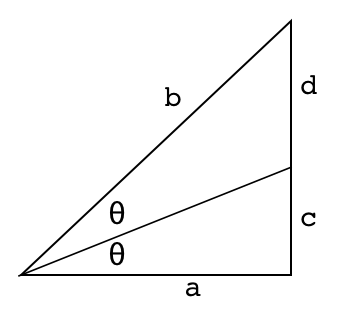
\includegraphics [scale=0.5] {angle_bisector_r1.png} \end{center}
Here we have chosen the first possibility.  We are in a position to prove an important theorem.
\subsection*{angle bisector theorem}
With reference to the figure above, we are to prove that
\[ \frac{d}{b} = \frac{c}{a} \]

Draw an altitude for the upper of the two small triangles, meeting the side of length $b$ at point $P$.
\begin{center} 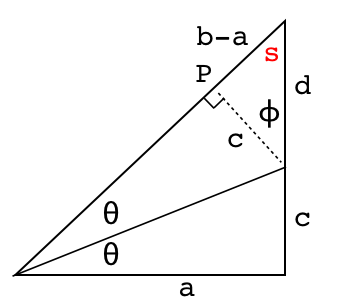
\includegraphics [scale=0.5] {angle_bisector_r2.png} \end{center}
By congruent triangles (the two triangles each with vertex angle $\theta$), the altitude has length $c$.

By the rules for complementary angles discussed above:
\[ 2 \theta + s = 90 = s + \phi \]

Hence, $2 \theta = \phi$.  We conclude that the smallest triangle at the top right of the figure is similar to the original.  By similar triangles, we form the equal ratios of the hypotenuse to the adjacent angle (either 
$\phi$ or $2 \theta$):
\[ \frac{d}{c} = \frac{b}{a} \]
This is rearranged simply to give
\[ \frac{d}{b} = \frac{c}{a} \]
which is what we were asked to prove.

$\square$

The result can be pushed a little further:
\[ \frac{a}{b} = \frac{c}{d} \]
Here's the key point
\[ \frac{a + b}{b} = \frac{c + d}{d} \]
\[ \frac{a + b}{c + d} = \frac{b}{d} = \frac{a}{c} \]
\begin{center} 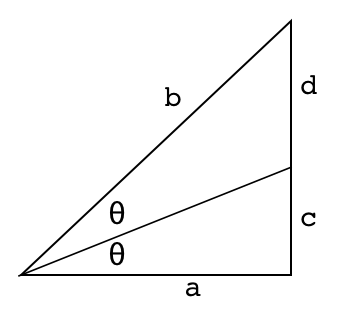
\includegraphics [scale=0.5] {angle_bisector_r1.png} \end{center}

which is a surprising result and becomes important in looking at Archimedes method for approximating the value of $\pi$.
 
\end{document}